\label{sec:register}
\begin{figure}[htbp]
\begin{center}
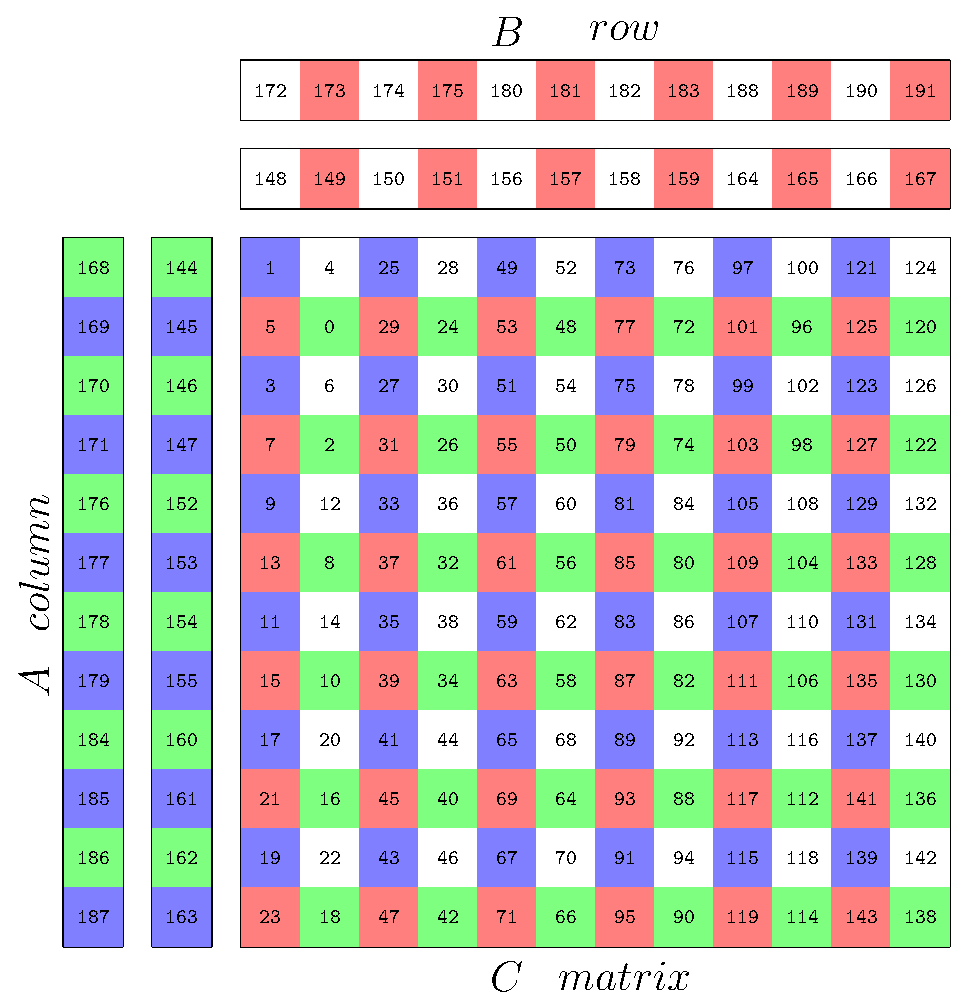
\includegraphics[scale=0.35]{reg_alloc}
\caption{\small Register allocation in SGEMM. Every number in a cell is a register index.
Different colors denote the mapping of register banks: green$\rightarrow$bank0,
    blue$\rightarrow$bank1, gray$\rightarrow$bank2, red$\rightarrow$bank3.}
\label{fig:reg}
\end{center}
\end{figure}
\subsection{Register Allocation}

To allocate registers for a $A$ column, $B$ row, and $C$ matrix block as in Algorithm~\ref{gemm}, we have three objectives:
correctness, no bank conflict, and tight register indices.
{\tt LDG.128} restricts four words alignment for registers.
Since NVIDIA GPU does not have $128$-bit registers, 
four consecutive $32$-bit registers {\tt RN}, {\tt RN+1}, {\tt RN+2}, and {\tt RN+3} will be an equivalence for a 128-bit
register.
%a $128$-bit load instruction ({\tt LDG.128}) writes the data to four consecutive $32$-bit registers {\tt RN}, {\tt RN+1}, {\tt RN+2}, and {\tt RN+3} given one destination register $RN$.
% in order to use $128$-bit load, one destination register $RN$ is given,
% results will be written to
% four $32$-bit registers: {\tt RN}, {\tt RN+1}, {\tt RN+2}, {\tt RN+3}.
We discover an undocumented restriction that \jli{$N$ must be dividable by $4$, what's N?},
% $N\mod4=0$
otherwise illegal instruction errors will be reported.
% It's not hard to understand this restriction,
The four words alignment restriction for {\tt LDG.128} simplifies hardware logic and cuts down power.
Since we use {\tt LDG.128} to load $A$ and $B$, there are two bank allocation choices under this restriction and Kepler's bank distribution (Table~\ref{tab:reg}).
We use four colors to represent the four banks respectively and show the register allocation when computing a $12 \times 12$ block of C in Figure~\ref{fig:reg}.
We assume allocating banks of $A$ as $\begin{bmatrix} 0 \\ 1  \end{bmatrix}$,
   banks of $B$ as $\begin{bmatrix} 2 & 3 \end{bmatrix}$ 
   as in Figure~\ref{fig:reg}, two choices are left for $C$,
$\begin{bmatrix} 1 & 2 \\ 3 & 0  \end{bmatrix}$ and
$\begin{bmatrix} 3 & 1 \\ 0 & 2  \end{bmatrix}$.
The $2\times2=4$ bank patterns of SGEMM are equivalent in performance, then we arbitrarily
choose $\begin{bmatrix} 0 \\ 1  \end{bmatrix}$ $\begin{bmatrix} 2 & 3 \end{bmatrix}$
    $\begin{bmatrix} 1 & 2 \\ 3 & 0  \end{bmatrix}$ for $A$, $B$ and $C$ respectively.
% We have $2\times2$ bank patterns for SGEMM, these four patterns are equivalent in performance,
%To allocate actual register index, we choose continuous register index so that register index do not get too big to exceed 255. 
For actual register index allocation, we choose continuous register indices to avoid exceeding $255$.
Every matrix block $C_{ij}$, column $A_i$ and row $B_j$ have different banks in Figure~\ref{fig:reg}, thus register bank conflicts are completely avoided.
% for example $C_{01}$'s color is white, $A_0$'s color is green and $B_1$'s color is red, .
